\section{Endliche Drehgruppen im dreidimensionalen Raum}
\begin{bem}
 Sei $W$ ein Untervektorraum mit $\dim W = 2$ im Vektorraum V mit $\dim V = 3$. Wenn $R$ eine Drehung in $\mathcal{O}(W)$ ist, dann kann $R$ zu einer Drehung in $\mathcal{O}(V)$ erweitert werden. Dazu wählen wir eine Basis $\{x_1,x_2,x_3\}$ von $V$ mit $x_1 \in W^{\perp}$ und $x_2,x_3 \in W$, sodass die Matrix $R$ durch \begin{center}
                                                                                                                                                                                                                                                                                                                                 $A=\begin{pmatrix}                                                                                                                                                                                                                                                                                                                                     
   1 && 0 && 0 \\
   0 && \cos(\theta) && -\sin(\theta) \\
   0 && \sin(\theta) && \cos(\theta)
   \end{pmatrix}
$                                                                                                                                                                                                                                                                                                                         \end{center}
repräsentiert wird.
\end{bem}
\begin{bem}
 Wenn wir jede Transformation $T$ aus einer Diederuntergruppe $\mathcal{H}^n_2$ zu einer Drehung in $\mathcal{O}(V)$ erweitern, dann erhalten wir eine Menge von Drehungen die eine Untergruppe von $\mathcal{O}(V)$ bildet und diese Untergruppe ist isomorph zu $\mathcal{H}^n_2$. Wir bezeichnen sie als Diedergruppe $\mathcal{H}^n_3$.
\end{bem}
\subsection{Platonische Körper}
 Da endliche Untergruppen von $\OR{2}$ Symmetriegruppen von regelmäßigen Polygonen sind, ist es naheliegend, dass wir uns nun mit regelmäßigen Polyedern beschäftigen. Es gibt genau 5 regelmäßige Polyeder, die sogenannten platonischen Körper. 
 
 Wenn wir ein regelmäßiges Polyeder am Ursprung des $\mathbb{R}^3$ ausrichten, dann sind die Drehungen die das Polyeder wieder in sich überführen eine endliche Untergruppe von $\OR{3}$. Auf diese Art entstehen drei unterschiedliche endliche Gruppen von Drehungen, denn der Würfel besitzt die gleiche Menge von Drehungen wie das Oktaeder und das Ikosaeder besitzt die gleiche Menge von Drehungen wie das Dodekaeder. Die folgende Illustration verdeutlicht warum dies der Fall ist.
 \\  \\
 \begin{center}
 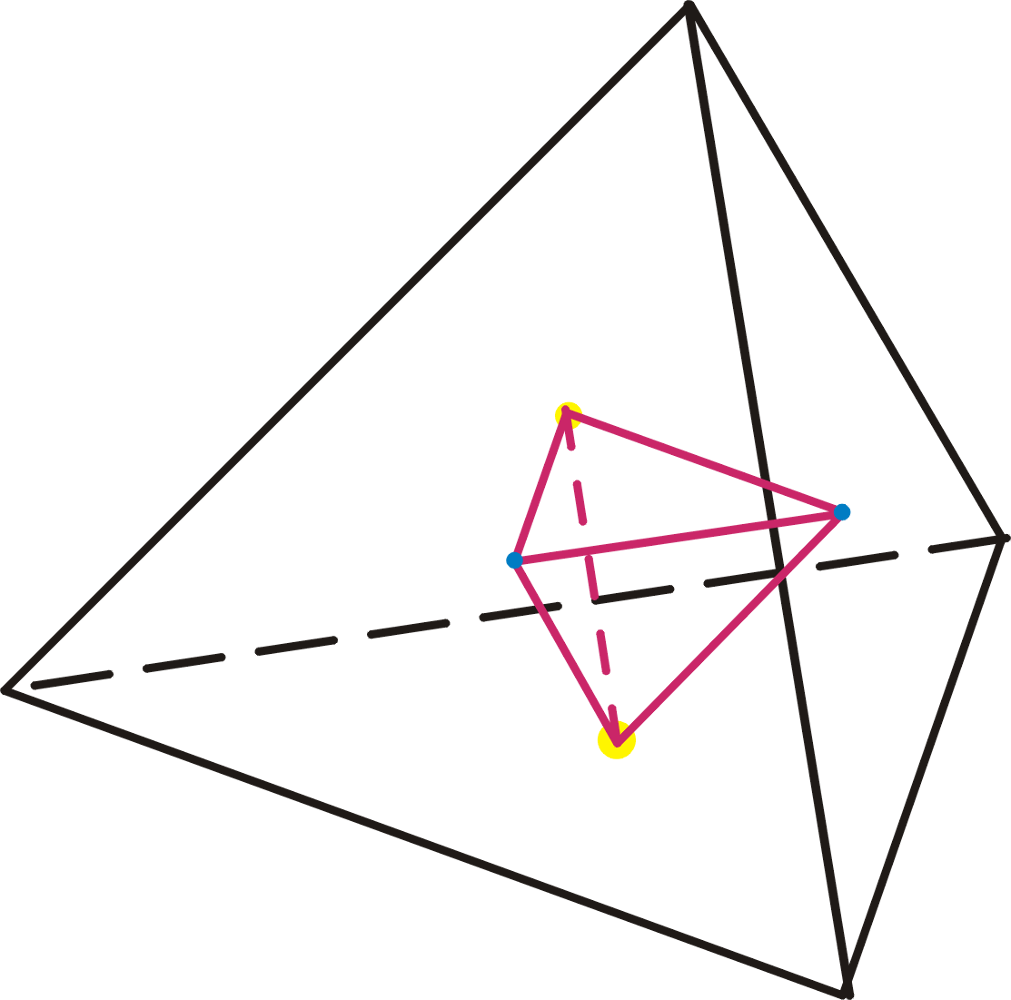
\includegraphics[height=110px]{./Grafiken/Duality_Tetra-Tetra.png} \ \
 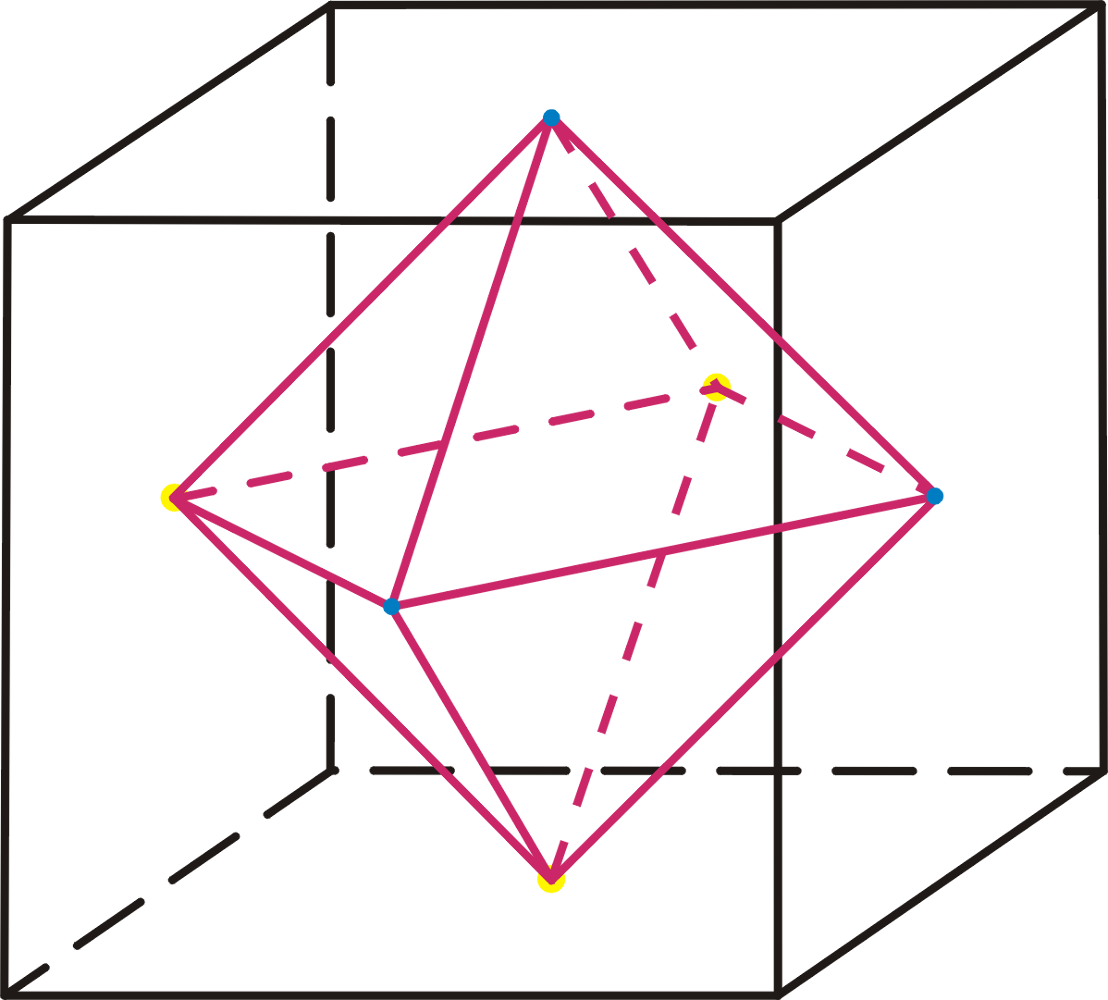
\includegraphics[height=110px]{./Grafiken/Duality_Hexa-Okta.png} \ \
 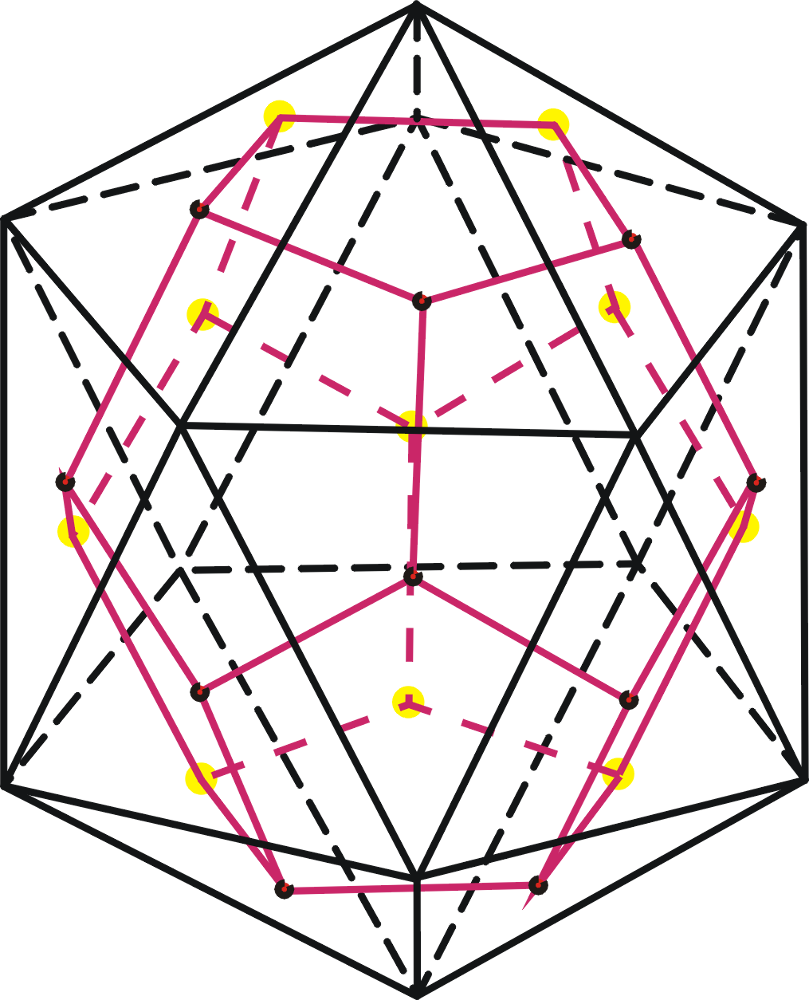
\includegraphics[height=110px]{./Grafiken/Duality_Iko-Dodek.png}
 \end{center}
 \newpage
Aus der Skizze lassen sich auch die Drehungen, die die Körper in sich überführen, leicht ablesen. Im nächsten Abschnitt nehmen wir an, dass die Schwerpunkte der Körper im Ursprung vom $\mathbb{R}^3$ liegen.

Zunächst betrachten wir die Untergruppe $\mathcal{T}$ der Drehungen von $\OR{3}$ des Tetraeders. Diese enthält
\begin{itemize}
  \item die Identität
  \item 8 Drehungen, um die Drehachsen zwischen einem Eckpunkte und dem Mittelpunkt der gegenüberliegenden Seite mit Drehwinkel $\frac{2}{3}\pi,\frac{4}{3}\pi$
  \item 3 Drehungen, um die Drehachsen zwischen den Mittelpunkten zweier gegenüberliegender Kanten mit Drehwinkel $\pi$
\end{itemize}
Es gilt somit $|\mathcal{T}|=4 \cdot 2 + 3 \cdot 1 +1 = 12$

Als nächstes betrachen wir die Untergruppe $\mathcal{W}$ der Drehungen von $\OR{3}$ des Würfels. Diese enthält
\begin{itemize} 
  \item die Identität
  \item 9 Drehungen, um die Drehachsen zwischen den Mittelpunkten zweier gegenüberliegender Seiten mit Drehwinkel $\frac{1}{2}\pi,\pi,\frac{3}{2}\pi$
  \item 8 Drehungen, um die Drehachsen zwischen zwei gegenüberliegenden Eckpunkten mit Drehwinkel $\frac{2}{3}\pi,\frac{4}{3}\pi$
  \item 6 Drehungen, um die Drehachsen zwischen den Mittelpunkten zweier gegenüberliegenden Kanten mit Drehwinkel $\pi$
\end{itemize}
Es gilt somit $|\mathcal{W}|=6 \cdot 1 + 4 \cdot 2 + 3 \cdot 3 +1 = 24$

Zuletzt betrachen wir die Untergruppe $\mathcal{I}$ der Drehungen von $\OR{3}$ des Ikosaeders. Diese enthält
\begin{itemize} 
  \item die Identität
  \item 24 Drehungen, um die Drehachsen zwischen zwei gegenüberliegendenden Eckpunkten mit Drehwinkel $\frac{2}{5}\pi,\frac{4}{5}\pi,\frac{6}{5}\pi,\frac{8}{5}\pi$
  \item 20 Drehungen, um die Drehachsen zwischen den Mittelpunkten zweier gegenüberliegender Seiten mit Drehwinkel $\frac{2}{3}\pi,\frac{4}{3}\pi$
  \item 15 Drehungen, um die Drehachsen zwischen den Mittelpunkten zweier gegenüberliegender Kanten mit Drehwinkel $\pi$
\end{itemize}
Es gilt somit $|\mathcal{I}|=15 \cdot 1 + 10 \cdot 2 + 6 \cdot 4 +1 = 60$
\begin{defi}
 Sei $E_3 \neq T \in \OR{3}$ eine Drehung, dann hat $T$ genau zwei Fixpunkte auf der Einheitskugel, nämlich die Schnittpunkte der Einheitskugel mit der Drehachse. Diese Punkte nennen wir die Pole der Drehung.
\end{defi}
\begin{lemma}
 Sei $\mathcal{G} \leq \OR{3}$, dann ist $\mathcal{G}$ eine Permutationsgruppe auf der Menge $\mathcal{P}$ ihrer Pole.
\end{lemma}
\begin{proof}
 Wenn $x \in \mathcal{P}$ ist, dann ist $x$ ein Pol einer Drehung $T \in \mathcal{G}$ mit $T \neq E_3$. Für jede Drehung $R \in \mathcal{G}$ wissen wir $Rx=RTx=(RTR^{-1})Rx$. Also ist $Rx$ ein Pol der Drehung $RTR^{-1}$ und es gilt $Rx \in \mathcal{P}$.
\end{proof}
\begin{bem}
 Wenn wir uns die Bahnen, die Ordnung der Stabilisatoren und die Anzahl der Pole einer Symmetriegruppe $\mathcal{G}$ mit Polmenge $\mathcal{P}$ anschauen, dann ergeben sich folgende charakteristische Werte.
 {%
\begin{center}
\begin{tabular}{l|cccccc}
$\mathcal{G}$ & $|\mathcal{G}|$ & $|\mathcal{P}|$ & Anzahl Bahnen & \multicolumn{3}{c}{Ordnung der Stabilisatoren}\\
\hline
$\mathcal{C}^n_3$ & $n$ & $2$ & $2$ & \ \ \ \ \ $n$ & \ \ \ \ \ \ $n$ & \\
$\mathcal{H}^n_3$ & $2n$ & $2n + 2$ & $3$ & \ \ \ \ \ $2$ & \ \ \ \ \ \ $2$ & $n$\\
$\mathcal{T}$ & $12$ & $14$ & $3$ & \ \ \ \ \ $2$ & \ \ \ \ \ \ $3$ & $3$\\
$\mathcal{W}$ & $24$ & $26$ & $3$ & \ \ \ \ \  $2$ & \ \ \ \ \ \ $3$ & $4$\\
$\mathcal{I}$ & $60$ & $62$ & $3$ & \ \ \ \ \ $2$ & \ \ \ \ \ \ $3$ & $5$
 \end{tabular}
 \end{center}
}%
\end{bem}
\begin{theorem}
 Haben $\mathcal{C}^n_3,\mathcal{H}^n_3,\mathcal{T},\mathcal{W}$ und $\mathcal{I}$ die gleichen Eigenschaften wie in Bemerkung 5.5, dann ist $\mathcal{C}^n_3,n\geq1;\mathcal{H}^n_3,n\geq2;\mathcal{T};\mathcal{W};\mathcal{I}$ eine komplette Liste aller endlichen Untergruppen von Drehungen aus $\OR{3}$.
\end{theorem}
\begin{proof}
 Sei $\mathcal{G}$ eine endliche Untergruppe bestehend aus Drehungen von $\OR{3}$ und $p \in \mathcal{P}$ ein Pol von $R \in \mathcal{G}$ beliebig, dann sei $Stab(p) := \{R\in \mathcal{G} | R(p)=p\}$ der Stabilisator eines Pols p von G und $R_p := \{R(p) | R \in G \}$ die zugehörige Bahn.
 
 Zunächst führen wir folgende Bezeichnungen eine
 \begin{center}
  $N:=|\mathcal{G}|$, $n_p:=|\mathcal{G}_p|=$ "`Bahnlänge"', $r_p:=|Stab(p)|$,
 \end{center}
dann gilt nach der Bahnenformel $N=r_p \cdot n_p$. Nach Definition eines Pols gilt $r_p > 1$, wenn $N > 1$, da die Identität immer in $Stab(p)$ enthalten ist. Außerdem hat $\mathcal{G}$ $r_p - 1$ Elemente mit Pol $p$ nach Definition des Stabilisators. Da jedes $T \in \mathcal{G}\backslash\{E_3\}$ zwei Pole hat, folgt:
\setcounter{equation}{0}
\begin{align}
 \sum_{p \in X}(r_p - 1)= 2(N-1)
\end{align}
Wenn zwei Pole $p$ und $p^{\#}$ in derselben Bahn liegen, dann folgt $\mathcal{G}_p=\mathcal{G}_{p^{\#}}$ und auch $N=r_p n_p=r_{p^{\#}} n_{p^{\#}}$. Wir können also Summanden von Polen, die in derselben Bahn liegen zusammenfassen. Wenn gilt $r_i=r_p$, falls $p\in B_i$, die Anzahl der verschiedenen Bahnen $m$ ist und $n_i:=|B_i|$, dann folgt aus $(1)$
\begin{align}
 &\sum_{i=1}^m n_i(r_i-1)=2(N-1) \\
 \Leftrightarrow &\underbrace{\sum_{i=1}^m \underbrace{(1-\frac{1}{r_i})}_{\substack{\geq \frac{1}{2}}}}_{\substack{\geq \frac{m}{2}}}=\underbrace{2-\frac{2}{N}}_{\substack{<2}}
\end{align}
Aus dieser Gleichung folgt, dass es höchstens 3 Bahnen geben kann, da $m \leq 3$. Wir möchten nun die drei Fälle überprüfen und schauen welche Drehgruppen wir dann vorliegen haben.

\textbf{Fall 1:} Es gilt $m=1$. Also existiert genau eine Bahn und es folgt aus Gleichung (3):
\begin{align*}
 \underbrace{2-\frac{2}{N}}_{\substack{\geq 1}} = \underbrace{1-\frac{1}{r_1}}_{\substack{<1}}
\end{align*}
Dies ist aber ein Widerspruch, sodass es nicht nur eine Bahn geben kann.

\textbf{Fall 2:} Es gilt $m=2$. Also existieren genau zwei Bahnen und aus (3) folgt:
\begin{align*}
 2-\frac{2}{N} &= 1-\frac{1}{r_1} + 1-\frac{1}{r_2} \\
 \frac{2}{N} &= \frac{1}{r_1} + \frac{1}{r_2}
\end{align*}
Da $N=r_i n_i$ gilt, muss $r_i \leq N$ gelten und somit folgt, dass $r_1 = r_2 = N$ und $n_1 = n_2 = 1$. Beide Bahnen haben die Länge 1 und daher gibt es nur zwei Pole $p$ und $p^{\#}$. Außerdem liegen sich beide Punkte auf der Einheitskugel gegenüber und sind Fixpunkte von G, das heißt die beiden Pole liegen auf einer Gerade durch den Ursprung. Daher kann die Gruppe G nur aus Drehungen um die Drehachse, die von $p$ und $p^{\#}$ gebildet wird, bestehen. Dies ist genau die Eigenschaft der Zyklischengruppe, daher gilt $\mathcal{G}=\mathcal{C}_3^n$.

\textbf{Fall 3:} Es gilt $m=3$. Aus (3) folgt dann:
\begin{align}
 \frac{2}{N} = \frac{1}{r_1} + \frac{1}{r_2} + \frac{1}{r_3} - 1
\end{align}
Wir sortieren die Bahnen so, dass $r_1 \leq r_2 \leq r_3$ gilt. Daraus folgt, dass $r_1 = 2$ sein muss, da für $r_i \geq 3$ die rechte Seite sonst kleiner Null wäre und es somit zu einem Widerspruch kommen würde. Mit Hilfe der obrigen Gleichung können wir feststellen, dass es nur vier weitere mögliche Kombinationen gibt $\{(2,2,n),(2,3,3),(2,3,4),(2,3,5)\}$.


$(2,2,n)$: Aus Gleichung (4) folgt, dass $N = 2n$ und $n_3=2$. Daher besteht die Bahn $B_3$ aus zwei Elementen $p, p^{\#}$. Das heißt, dass jedes Element von $\mathcal{G}$ die Pole $p,p^{\#}$ festhält oder sie vertauscht. Daher müssen sich beide Pole gegenüberliegen und die Elemente aus $\mathcal{G}$ sind entweder Drehungen um die Drehachse $d$ durch die beiden Pole $p,p^{\#}$ oder Drehspiegelungen mit Drehachse $d$ um den Winkel $\pi$ und Spiegelebene $d^{\perp}$. Daher besitzt G genau die Eigenschaften der Diedergruppe und es gilt $\mathcal{G} = \mathcal{H}_3^n$. Die Eckpunkte und die Mittelpunkte der Seiten entsprechen dann den übrigen Polen. 


$(2,3,3)$: Aus Gleichung (4) folgt, dass $N = 12$ und $n_1 = 6, n_2 = 4, n_3 = 4$ gilt. Die Pole der Bahn $B_2$ sind die Eckpunkte eines Tetraeders $T$ und $\mathcal{G}$ ist die Drehgruppe $\mathcal{T}$. Außerdem gilt, dass
\begin{align*}
n_1 = \# Kanten(T),n_2 = \# Eckpunkte(T),n_3 = \# \text{Flächen}(T)
\end{align*}


$(2,3,4)$: Aus Gleichung (4) folgt, dass $N = 24$ und $n_1 = 12, n_2 = 8, n_3 = 6$ gilt. Die Pole der Bahn $B_2$ sind die Eckpunkte eines Würfels $W$ und $\mathcal{G}$ ist die Drehgruppe $\mathcal{W}$. Außerdem gilt, dass
\begin{align*}
n_1 = \# Kanten(W),n_2 = \# Eckpunkte(W),n_3 = \# \text{Flächen}(W)
\end{align*}


$(2,3,5)$: Aus Gleichung (4) folgt, dass $N = 60$ und $n_1 = 30, n_2 = 20, n_3= 12$ gilt. Die Pole der Bahn $B_3$ sind die Eckpunkte eines Ikosaeders $I$ und $\mathcal{G}$ ist die Drehgruppe $\mathcal{I}$. Außerdem gilt, das
\begin{align*}
n_1 = \# Kanten(I),n_2 = \# \text{Flächen}(I),n_3 = \# \text{Eckpunkte}(T)
\end{align*}
\end{proof}
